\pdfminorversion=4

\documentclass{beamer}  %add [handout] to eliminate
\usetheme{Boadilla}
%\usefonttheme{structurebold}
\usecolortheme{beaver}

\usepackage{times}
\usepackage[english]{babel}
\usepackage{pgf,pgfarrows,pgfnodes,pgfautomata,pgfheaps}
\usepackage{amsmath,amssymb}
\usepackage[latin1]{inputenc}
\usepackage{algorithm}
\usepackage{algorithmicx}
\usepackage{hyperref}
\usepackage{graphicx}
\usepackage{multicol}


\usepackage{makeidx}
\usepackage{newtxtext,newtxmath}% Puts text in times new roman
%\usepackage{mathptmx}
\usepackage{latexsym}
\usepackage{epsfig}
\usepackage{color}
\usepackage{enumerate}

\usepackage{ulem}%for cross out text

%\setbeamercovered{dynamic}
\setbeamercovered{transparent=0}
%\setbeamertemplate{footline}{\insertframenumber/\inserttotalframenumber}
\setbeamertemplate{navigation symbols}{}


\newcommand{\Fan}[1]{\it {\color{green}[Notes for instructor: #1]}}
\newcommand{\bc}[1]{{\color{blue} #1}}
\newcommand{\rc}[1]{{\color{red} #1}}

\newcommand{\ml}{\textsc{Matlab} }
\newcommand{\calE}{\mathcal{E}}
\newcommand{\calI}{\mathcal{I}}
\renewcommand{\L}{\mathcal{L}}
\newcommand{\R}{\mathbb{R}}
\newcommand{\E}{\mathbb{E}}
\newcommand{\ds}{\displaystyle}

\renewcommand{\and}{\qquad \text{and}\qquad}
\newcommand{\zt}{\mathcal{Z}}
\newcommand{\D}{\mathbb{D}}
\newcommand{\C}{\mathbb{C}}

\usepackage{textpos}

%--------------------------------------------------------------------
\title[DDMR by Wiener Projection]{Data-driven Model Reduction by Wiener Projection}
\subtitle{}
\author[McBride]{Jared McBride}
\institute[Applied Math @ Arizona]{
$\quad$ \\
Applied Mathematics\\
University of Arizona
}
\date[9/18/2020]{Sept 18, 2020}
%--------------------------------------------------------------------

\addtobeamertemplate{frametitle}{}{%
\begin{textblock*}{15mm}(.74\textwidth,-0.72cm)

\includegraphics[height=0.6cm]{fig/logo-AM.png}
\end{textblock*}}

\usebackgroundtemplate{
\includegraphics[width=\paperwidth,height=\paperheight]{fig/logo-cover-AM.png}}

\begin{document}
\begin{frame}
  \titlepage
\end{frame}

\usebackgroundtemplate{
\includegraphics[width=\paperwidth,height=\paperheight]{fig/logo-bottom.png}}

%%%%%%%%%%%%%%%%%%%%%%%%%%%%%%%%%%%%%%%%%%%%%%%%%%%%%%%%%%%%%%%%%%%%%%%%%%%%%%%%%%%%%%%

\begin{frame}{Outline}
	\tableofcontents
\end{frame}



%%%%%%%%%%%%%%%%%%%%%%%%%%%%%%%%%%%%%%%%%%%%%%%%%%%%%%%%%%%%%%%%%%%%%%%%%%%%%%%%%%%%%%%
\section{The Problem}
%%%%%%%%%%%%%%%%%%%%%%%%%%%%%%%%%%%%%%%%%%%%%%%%%%%%%%%%%%%%%%%%%%%%%%%%%%%%%%%%%%%%%%%

\begin{frame}{The Problem}
Many important models today contemplate
\begin{itemize} 
\item \rc{large number of degrees of freedom} 
\item across many orders of magnitude in space and time, without sharp scale separation.
\end{itemize}

{\small 
	\textit{Examples: Power flow on large grids, neural activity in the brain, weather forecasting, etc.}
}

\bigskip

Some tasks require \rc{repeated model runs} such as for 
\begin{itemize}
	\item Uncertainty quantification
	\item Optimization and control
\end{itemize}

\bigskip

Commonly, only a relatively \bc{small} number of variables are of direct interest or even observable.
\end{frame}

%%%%%%%%%%%%%%%%%%%%%%%%%%%%%%%%%%%%%%%%%%%%%%%%%%%%%%%%%%%%%%%%%%%%%%%%%%%%%%%%%%%%%%%
\section{Goal and Difficulties}
%%%%%%%%%%%%%%%%%%%%%%%%%%%%%%%%%%%%%%%%%%%%%%%%%%%%%%%%%%%%%%%%%%%%%%%%%%%%%%%%%%%%%%%

\begin{frame}{Goal and Difficulties}
	The \textbf{goal} is then to find reduced order models, which include only the variables of interest (resolved variables), capable of \bc{finite time forecasting} as well as reproducing \bc{long-time statistics} like correlation functions and marginals of stationary distributions, at \emph{lower computational costs}.
	
	\bigskip 
	
	How can the effect of unresolved variables be approximated by using the resolved variables and \emph{stochastic terms}. 
	
	\bigskip
	
	
 Unlike under situations with sharp scale separation, 
 \begin{itemize}
 	\item memory (marginals of Markov process may not be Markov) and 
 	\item noise effects 
 \end{itemize} must be accounted for in many applications. 







\end{frame}
%%%%%%%%%%%%%%%%%%%%%%%%%%%%%%%%%%%%%%%%%%%%%%%%%%%%%%%%%%%%%%%%%%%%%%%%%%%%%%%%%%%%%%%
%%%%%%%%%%%%%%%%%%%%%%%%%%%%%%%%%%%%%%%%%%%%%%%%%%%%%%%%%%%%%%%%%%%%%%%%%%%%%%%%%%%%%%%
\section{Background}
%%%%%%%%%%%%%%%%%%%%%%%%%%%%%%%%%%%%%%%%%%%%%%%%%%%%%%%%%%%%%%%%%%%%%%%%%%%%%%%%%%%%%%%


%%%%%%%%%%%%%%%%%%%%%%%%%%%%%%%%%%%%%%%%%%%%%%%%%%%%%%%%%%%%%%%%%%%%%%%%%%%%%%%%%%%%%%%
\subsection{The Wiener Filter}
%%%%%%%%%%%%%%%%%%%%%%%%%%%%%%%%%%%%%%%%%%%%%%%%%%%%%%%%%%%%%%%%%%%%%%%%%%%%%%%%%%%%%%%

\begin{frame}{Wiener Filter}
	Given two stationary processes $\textbf{x}_n$,$\textbf{y}_n$ The Wiener Filter computes a \emph{linear least square estimate} $\hat{\textbf{y}}_n$ of a process $\textbf{y}_n$ given  $\textbf{x}_n$, for this reason  
	\begin{itemize}
		\item $\textbf{y}_n$ is called the signal,
		\item $\textbf{x}_n$ are called the predictors.
	\end{itemize}

	This means we seek an $h$ such that
	$$\E\|\textbf{y}_n - (\textbf{x}\star h)_n\|^2 = \text{minimum}$$
	
	In our case we want to require $h_n$ to be 
	\begin{itemize}
		\item causal (meaning $h_n=0$ for $n<0$)
		\item rapid decay (so that efficiency is gained)
	\end{itemize}
	
\end{frame}



\begin{frame}{Wiener Filter}{Causal Solution}
	Basically give the spectral density of  ${\textbf{yx}}$, $S_{\textbf{x}}(z)$, and the cross spectral density of ${\bf y}$ and ${\bf x}$, $S_{\textbf{yx}}(z)$ The causal solution is obtained by the formula below.
	$$H(z) = \left\{S_{\textbf{yx}}(z){S^+}^{-1}_{\textbf{x}}(z)\right\}_+ {S^-}^{-1}_{\textbf{x}}(z)$$
	Here ${S^+}$ and ${S^-}$ form a special factorization of $S_x$ such that $S^+(z) = S^{-*}(z^{-*})$,
	$$S(z) =S^+(z)S^-(z)\qquad \text{for }z\in \partial\D$$
	and $S^-(z)$ is minimum phase, meaning all it's poles and zeros are strictly inside the unit circle. This makes  $S^-(z)$ a causal and casually invertable LTI system. 
\end{frame}

%%%%%%%%%%%%%%%%%%%%%%%%%%%%%%%%%%%%%%%%%%%%%%%%%%%%%%%%%%%%%%%%%%%%%%%%%%%%%%%%%%%%%%%
\subsection{Spectral Factorization}

%%%%%%%%%%%%%%%%%%%%%%%%%%%%%%%%%%%%%%%%%%%%%%%%%%%%%%%%%%%%%%%%%%%%%%%%%%%%%%%%%%%%%%%
\begin{frame}{Spectral Factorization}{More specific}
	
	\begin{block}{our favorite version of Spectral Factorization Theorem}
		If $\textbf{y}$ is a mean zero, stationary, discrete time stochastic $d$-vector-valued process that admits a rational $z$-spectrum $S_{\textbf{y}}$ analytic on some annulus containing the unit circle,  and $$S_{\textbf{y}} > 0 \qquad \text{everywhere on } \partial\D.$$ Then there exists matrix functions $S^+(z)$ and $S^-(z)$, such 
		\begin{itemize}
			\item $S^+(z)$ is a $d\times d$ rational matrix function that is analytic on and inside the unit circle,
			\item ${S^+}^{-1}(z)$ is analytic on and inside the unit circle.
			\item $S^-(z) = S^{+*}(z^{-*})$ and 
			\item $S(z) =S^+(z)S^-(z)$.	
		\end{itemize}
	\end{block}
	
\end{frame}
%%%%%%%%%%%%%%%%%%%%%%%%%%%%%%%%%%%%%%%%%%%%%%%%%%%%%%%%%%%%%%%%%%%%%%%%%%%%%%%%%%%%%%%
\begin{frame}{Spectral Factorization}{More specific}
Notice that the factorization if non unique in this form, since is $U(z)$ is unitary on $\partial \D$ and $S^-(z)$ is a spectral factor of $S(z)$ then so is $U(z)S^-(z)$.

\bigskip

It would be nice to leverage this to improve performance. (possible future work)

\end{frame}
%%%%%%%%%%%%%%%%%%%%%%%%%%%%%%%%%%%%%%%%%%%%%%%%%%%%%%%%%%%%%%%%%%%%%%%%%%%%%%%%%%%%%%%
\begin{frame}{Spectral Factorization}{Numerical}
	
	Most Numerical algorithms assume $S(z)$ is rational and has the form of a \emph{Laurent Polynomial} meaning it may be written as $$S(z) = \sum_{n=-m}^m c_nz^{-n}\qquad \text{with }c_n = c_{-n}^*.$$
	If this is assumed it may be shown that 
	$$S^+(z) = \sum_{n=1} L_n z^{n} \and S^-(z) = \sum_{n=1} L_n^* z^{-n}$$

	Algorithms that use Toeplitz matrices.
	\begin{itemize}
		\item Schur
		\item Levinson-Durbin
	\end{itemize}
	Algorithms that use State Space formulations.
	\begin{itemize}
		\item Riccati Equation
		\item Kalman Filter
		\item Chadrasekhar-Kailath-Morf-Sidhu (CKMS)
	\end{itemize}
\end{frame}

%%%%%%%%%%%%%%%%%%%%%%%%%%%%%%%%%%%%%%%%%%%%%%%%%%%%%%%%%%%%%%%%%%%%%%%%%%%%%%%%%%%%%%%



%%%%%%%%%%%%%%%%%%%%%%%%%%%%%%%%%%%%%%%%%%%%%%%%%%%%%%%%%%%%%%%%%%%%%%%%%%%%%%%%%%%%%%%
\section{The Wiener Projection}
%%%%%%%%%%%%%%%%%%%%%%%%%%%%%%%%%%%%%%%%%%%%%%%%%%%%%%%%%%%%%%%%%%%%%%%%%%%%%%%%%%%%%%%

\begin{frame}{This Approach}
Given a full model
$$X_n = F(X_n)$$
with resolved variables collected in $x_n$,
select functions $\psi^{(i)}(x)$ (informed by model) on reduced state variables (resolved variables).
$$\psi(x) = \Big(\psi^{(0)}(x)\Big|\psi^{(1)}(x)\Big|\cdots\Big|\psi^{(\nu)}\Big)
\qquad\text{and}\qquad\psi_k = \psi(x_k).$$
$\psi_k$ are our predictors, $x_k$ is the signal, two stationary stochastic processes. Use WF to find LTI filter to approximate $X_k$ by $\psi_k$ optimally. This forms a ``reduced'' model, closed in the variables of interest.

\begin{equation*}
\boxed{x_{n+1} =  \sum_{k=0}^\infty \psi_{k}\cdot h_{n-k} + \xi_{n+1}}
\end{equation*}
We use the data to infer $h_{k}$ (WF) and $\xi_{n}$.

\end{frame}

\begin{frame}{This Approach}
	Why ``reduced''?

	If $h_k$ doesn't decay well, what do we gain?
	
	Let $y_n = \sum_{k=0}^\infty \psi_{k}\cdot h_{n-k}$ be an auxiliary variable.
	
	If we could take the $z$-transform of both sides we would get $$Y(z) = \Psi(z)\cdot H(z)$$ further if had had a good rational approximation $H(z) = A(z)/B(z)$ we could write 
	$Y(z)A(z) = \Psi(z)\cdot B(z)$ and 
	$$ y_n+a_1y_{n-1} + \dots +  a_py_{n-p}= \psi_{n-p}\cdot b_0 + \psi_{n-p+1}\cdot b_1 + \dots \psi_{n-p+q}\cdot b_q$$
	where $A(z) = z^p + a_1z^{p-1}+\dots+a_{p-1}z^{1}$ and $B(z) = b_0 + b_1z^{1}+\dots+b_qz^{q}$

\end{frame}

%%%%%%%%%%%%%%%%%%%%%%%%%%%%%%%%%%%%%%%%%%%%%%%%%%%%%%%%%%%%%%%%%%%%%%%%%%%%%%%%%%%%%%%

\begin{frame}{How to solve}
	Dr. Kevin Lin and Dr. Fei Lu solves the "WF" ($a$ and $b$) in time domain, using an numerical optimization optimization algorithm. 
	
	\bigskip
	
	This study investigates computing the Wiener filter by \emph{spectral methods} (that is, employing information like the power spectra $S_{yx}$ and $S_{x}$).  This is a direct method requiring no iterative optimization.
	
	\bigskip
	
	Advantages:
	\begin{itemize}
		\item Quicker
		\item more accurate (?)
	\end{itemize}
\end{frame}


%%%%%%%%%%%%%%%%%%%%%%%%%%%%%%%%%%%%%%%%%%%%%%%%%%%%%%%%%%%%%%%%%%%%%%%%%%%%%%%%%%%%%%%
\section{Numerical Impimentation: Examples}
%%%%%%%%%%%%%%%%%%%%%%%%%%%%%%%%%%%%%%%%%%%%%%%%%%%%%%%%%%%%%%%%%%%%%%%%%%%%%%%%%%%%%%%
\begin{frame}{WF Example: AR(2) Signal, Filtered, Ad. WN}
	Let us consider again the stationary autoregressive process of order 2,
	$$y_n = (r_1+r_2)y_{n-1} - r_1r_2 y_{n-2} + u_n , \qquad \text{for } n > -\infty$$
	for $r_1,r_2 \in \{z : |z|<1\}$.
	This time however, we define the observations to be the signal $y$ operated upon by a finite impulse response time invariant filter $w$ with additive white noise.
	$$x_n = (w * y)_n + v_n, \qquad \text{for } n > -\infty.$$
	
	For simplicity let $$ w = (\dots,0,\fbox{1},w_1, w_2,0,\dots),$$
	where the box indicate the element indexed by 0 and $w_1,w_2 \in \R$, then write
	$$W(z) = \sum_{k = -\infty}^\infty w_k z^{-k} = 1 + w_1 z^{-1} + w_2 z^{-2}.$$
	
\end{frame}	
\begin{frame}{WF Example: AR(2) Signal, Filtered, Ad. WN}
	Here is a run, with $r_1,r_2 = -0.2, 0.9$, $w_1,w_2 = -0.1, 5$, and $\sigma_{\textbf{v}} = 1.1$. The trajectory has $10^6$ steps after discarding $10^3$ steps. 
	
	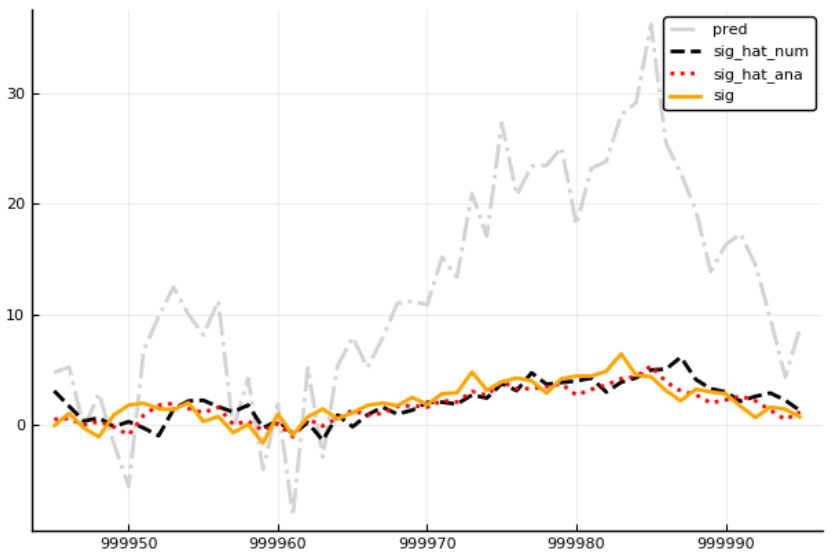
\includegraphics[scale=.33]{fig/figAR2F_ts.png}
	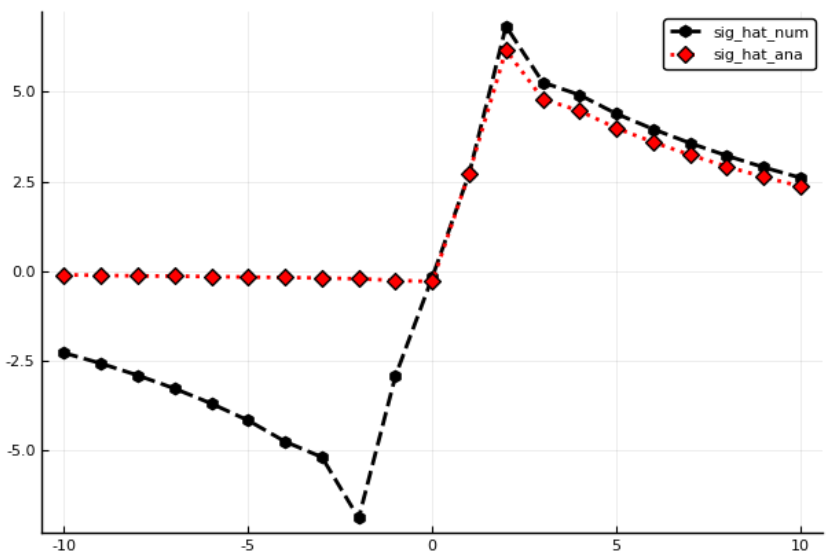
\includegraphics[scale=.33]{fig/figAR2F_cov.png}
	
	Left: A window of the time series for the signal (orange), the predictors (light gray), the estimated signal using the analytic and numerical Wiener filter (red, black). 
	
	Right: The covariance between errors (red from analytic filter, black from numerical) and predictors (observations). \\
\end{frame}


\begin{frame}{WF Example: AR(2) Signal, Filtered, Ad. WN}
	New results! The problem was in the function used to estimate the cross spectrum. It was a subtle bug I didn't find till I worked with complex-valued time series, in which case the bug was more apparent.  
	
	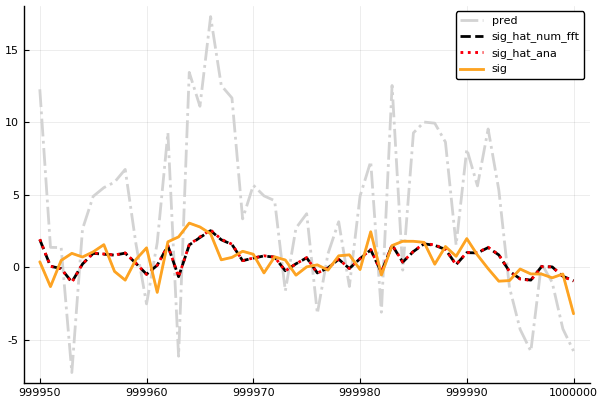
\includegraphics[scale=.33]{fig/figAR2F_ts_new.png}
	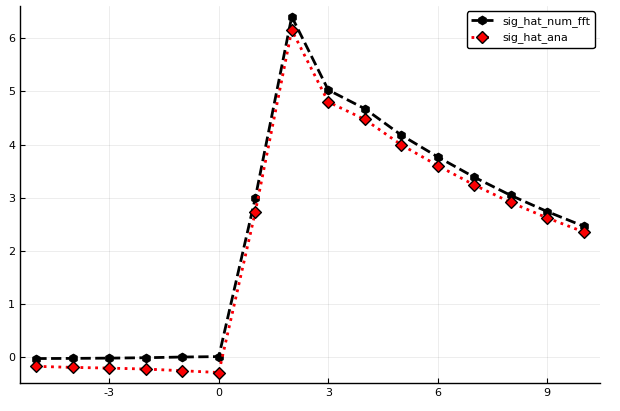
\includegraphics[scale=.33]{fig/figAR2F_cov_new.png}
	
	Left: A window of the time series for the signal (orange), the predictors (light gray), the estimated signal using the analytic and numerical Wiener filter (red, black). 
	
	Right: The covariance between errors (red from analytic filter, black from numerical) and predictors (observations). \\
\end{frame}

%%%%%%%%%%%%%%%%%%%%%%%%%%%%%%%%%%%%%%%%%%%%%%%%%%%%%%%%%%%%%%%%%%%%%%%%%%%%%%%%%%%%%%%

\begin{frame}{MR Example: Nonlinear Langevin}{Double-welled Potential}
	
		In this example we consider the stochastic, over-damped Langevin equation with a double-welled potential $V(x) = \frac{1}{4}(x^2 - 1)^2$. So, we consider the following SDE. 
		$$dX_t = -X_t(X_t^2 - 1)dt + dB_t$$
		To find a numerical solution we first use the Euler-Maruyama scheme 
		$$X_{n+1} = X_n - h X_n(X_n^2 - 1) + e_n$$
		here $$e_n \sim (B_{t_{n+1}}-B_{t_{n}}) \sim N(0,h) \sim \sqrt{h} N(0,1).$$
		
		Now we generate the sample path.
\end{frame}


\begin{frame}{MR Example: Nonlinear Langevin}{Double-welled Potential}
	The full was generated by Euler-Maruyama 150 million ($1.5\cdot 10^8$) steps, ($1.5\cdot 10^5$ secs at a time step of $10^{-3}$) $\sigma = .35$ we discarded $10^7$
	
	The observations seen below are every $100$th point.
	
	\bigskip
	
	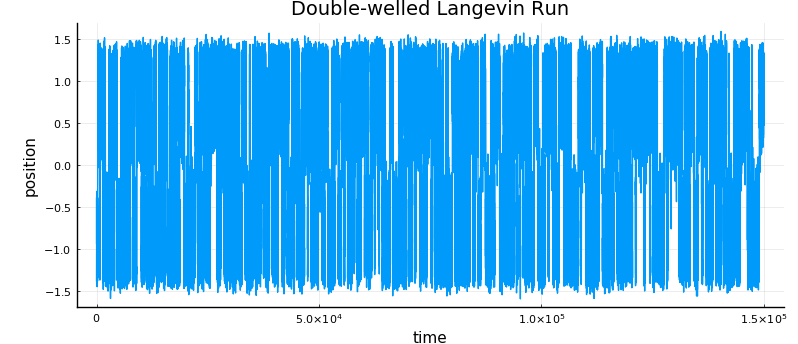
\includegraphics[scale=.6]{fig/RunNLL.png}
\end{frame}


\begin{frame}{MR Example: Nonlinear Langevin}{Double-welled Potential}
		Recall the original model was
		$$X_{n+1} = X_n - h X_n(X_n^2 - 1) + e_n$$
		so we will choose $\psi(x) = [x;x^3]$
		We feed these into the Wiener filter function and get the WF.
		
		
\end{frame}



%%%%%%%%%%%%%%%%%%%%%%%%%%%%%%%%%%%%%%%%%%%%%%%%%%%%%%%%%%%%%%%%%%%%%%%%%%%%%%%%%%%%%%%
\section{KSE}
%%%%%%%%%%%%%%%%%%%%%%%%%%%%%%%%%%%%%%%%%%%%%%%%%%%%%%%%%%%%%%%%%%%%%%%%%%%%%%%%%%%%%%%
\begin{frame}{Karumoto-Sivashinsky Equation}
	In one demnsional space is 
	$$u_t + uu_x + u_{xx} + u_{xxxx} = 0,\qquad t \in [0,\infty), x \in [o,L]$$
	 
In Fourier coefficients this is 
$$\dot{v}_k = -\frac{iq_k}{2}\sum_l v_l v_{k-l} + (q_k^2 - q^4_k)v_k, \qquad q_k = \frac{2\pi k}{L}$$
this is now an ODE in the Fourier modes, we now use a numerical scheme to solve this ODE. 

\end{frame}

\begin{frame}{Karumoto-Sivashinsky Equation}
	These ODE's tend to be stiff so we use an exponential time differencing (ETD) scheme to solve them. This scheme is paired up with an RK4 method.  
	
	 
		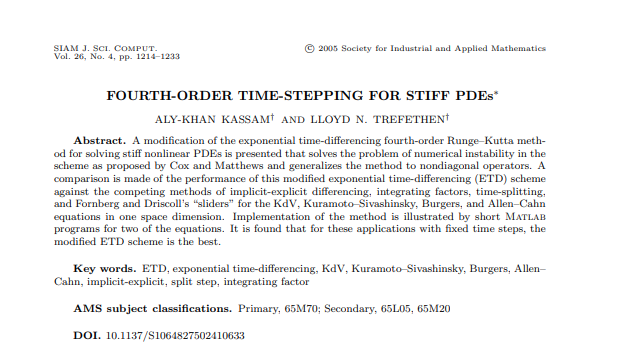
\includegraphics[scale=.7]{fig/ETDRK41.png}
\end{frame}

\begin{frame}{Karumoto-Sivashinsky Equation}
\begin{minipage}{.5\textwidth}
	This introduces the full model of the form
$$V_{n+1} = F(V_n)$$
Where $F$ steps the vector $V_n = (v_k^n;\: n\in \mathbb{Z})$ forward in time. Generally, because of the decay of the Fourier modes we consider only the first so many modes, about 100.

Displayed used 96 modes, $10^8$ I discarded half, The time step is $10^3.$ 
	\end{minipage}\begin{minipage}{.5\textwidth}
	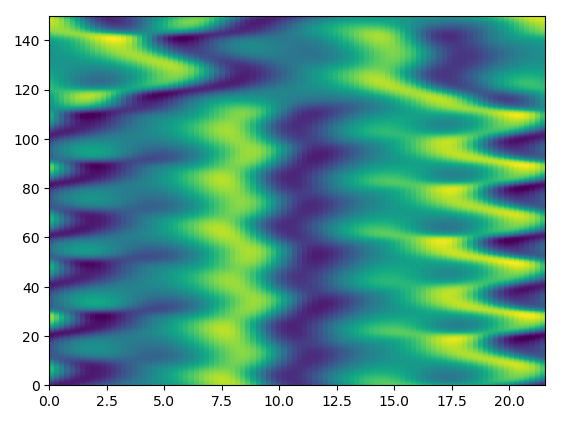
\includegraphics[scale=.45]{fig/KSE_mine.png}
\end{minipage}
\end{frame}

%%%%%%%%%%%%%%%%%%%%%%%%%%%%%%%%%%%%%%%%%%%%%%%%%%%%%%%%%%%%%%%%%%%%%%%%%%%%%%%%%%%%%%%
\section{Difficulties}
%%%%%%%%%%%%%%%%%%%%%%%%%%%%%%%%%%%%%%%%%%%%%%%%%%%%%%%%%%%%%%%%%%%%%%%%%%%%%%%%%%%%%%%
\begin{frame}{Difficulties}
	The theoretically two ingredients are $S_{X\Psi}(z)$ and $S_{X}(z)$. Rather, $S_{X\Psi}(z)$ and $S^-_{X}(z)$ ($S^+_{X}(z)$ $S^-_{X}(z)$ derives from we need What we have is data. 
	
	These can be difficult to estimate. Here is an illustration: 
	
\end{frame}		

\begin{frame}{WF: AR(2) Signal, Filtered, Ad. WN}{Estimating $S_{X\Psi}(z)$}
	Observe that 
	$$S_{\textbf{yx}}(z) = S_{\textbf{y}}(z)W^*(z^{-*}) \and S_{\textbf{x}} = W(z)S_{\textbf{y}}(z)W^*(z^{-*}) + \sigma_{\textbf{v}}^2.$$
	So, 
	\begin{align*}
	S_{\textbf{yx}}(z) &= \frac{1 + w_1 z + w_2 z^{2}}{ (1 - r_1z^{-1})(1 - r_2z^{-1})(1 - r_1^*z)(1 - r_2^*z)}\\
	\end{align*}
	
	Numerically this is processed in 
	\begin{enumerate}
		\item estimate cross covariances
		\item smooth these
		\item take $z$-transform (fft)
	\end{enumerate}
	
\end{frame}
	
	
\begin{frame}{WF: AR(2) Signal, Filtered, Ad. WN}{Estimating $S_{X\Psi}(z)$}
Here's a snippet:


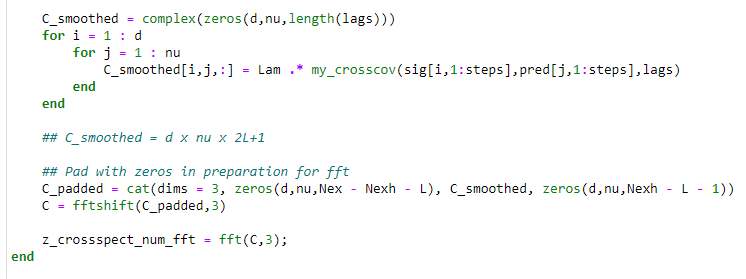
\includegraphics[scale=.6]{fig/Spectsigpred_code.PNG}
	
\end{frame}
	

\begin{frame}{WF: AR(2) Signal, Filtered, Ad. WN}{Estimating $S_{X\Psi}(z)$}
	Here's the result:
	
	
	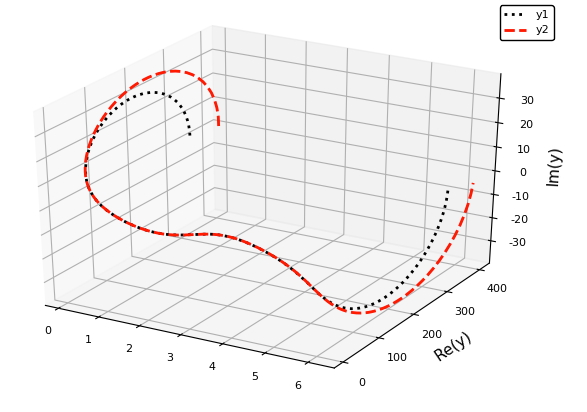
\includegraphics[scale=.6]{fig/spectsigpred.PNG}
	
\end{frame}

\begin{frame}{WF: AR(2) Signal, Filtered, Ad. WN}{Estimating $S^-_{\Psi}(z)$}
	For this, analytically we have we have 
	\begin{align*}
	S_{\textbf{x}}(z) &=\frac{w_2 + \sigma_{\textbf{v}}^2r^*_1r^*_2}{\rho_1^*\rho_2^*}\cdot \frac{(1 - \rho_1z^{-1})(1 - \rho_2z^{-1})(1 - \rho_1^*z)(1 - \rho_2^*z)}{(1 - r_1z^{-1})(1 - r_2z^{-1})(1 - r_1^*z)(1 - r_2^*z)}
	\end{align*} 
	
	Numerically this is processed in 
	\begin{enumerate}
		\item estimate autocovariance
		\item smooth this
		\item feed it into factorizing script
		\item take fft
	\end{enumerate}
	
\end{frame}


\begin{frame}{WF: AR(2) Signal, Filtered, Ad. WN}{Estimating $S_{X\Psi}(z)$}
	Here's a snippet:
	
	
	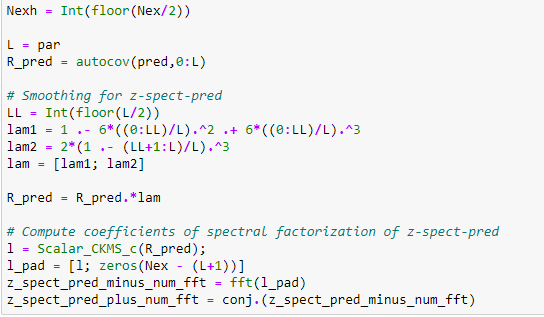
\includegraphics[scale=.6]{fig/spectpred_code.PNG}
	
\end{frame}


\begin{frame}{WF: AR(2) Signal, Filtered, Ad. WN}{Estimating $S_{X\Psi}(z)$}
	Here's the result:
	
	
	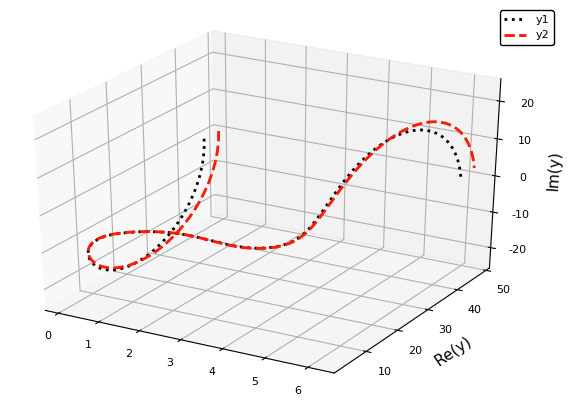
\includegraphics[scale=.6]{fig/spectpred.PNG}
	
\end{frame}


\section{Conclusions}
%%%%%%%%%%%%%%%%%%%%%%%%%%%%%%%%%%%%%%%%%%%%%%%%%%%%%%%%%%%%%%%%%%%%%%%%%%%%%%%%%%%%%%%



\begin{frame}
Thank you!
\end{frame}


\end{document}




